\documentclass[hyperref=colorlinks]{beamer}
\mode<presentation>
\usetheme{iclpt}
\setbeamertemplate{navigation symbols}{}
\setbeamertemplate{headline}{
  \begin{beamercolorbox}[leftskip=.2cm,rightskip=.2cm,topskip=.2cm,ht=1.1cm,dp=0.1cm,wd=\textwidth]{institute in head/foot}
    
\includegraphics[height=1cm]{icl.pdf}
    \hfill
    
\includegraphics[height=1cm]{../Pics/CMS-Color.pdf}
  \end{beamercolorbox}
}
\setbeamertemplate{footline}{
  \begin{beamercolorbox}[ht=.35cm,dp=0.2cm,wd=\textwidth,leftskip=.3cm]{author in head/foot}%
    \begin{minipage}[c]{5cm}%
      \usebeamerfont{author in head/foot}
      \insertshortauthor 
      \insertshorttitle
    \end{minipage}\hfill%
    \hfill
    \hypersetup{linkcolor=}
    \insertframenumber{} / \textcolor{beamer@iclightblue}{\ref{lastframe}}
    %\hfill
    \begin{minipage}{6cm}
      \hfill
      %\insertshorttitle
    \end{minipage}
  \end{beamercolorbox}%
}

\usepackage{color}
\usepackage{tabularx,colortbl}
\usepackage{graphicx}
\usepackage{pdfpages}
\usepackage{feynmp}
\usepackage{rotating}
\usepackage{moresize}
\usepackage{xcolor,colortbl}
\usepackage{tikz}
\usetikzlibrary{arrows,shapes,backgrounds}
\DeclareGraphicsRule{*}{mps}{*}{}

\tikzset{
  invisible/.style={opacity=0},
  visible on/.style={alt={#1{}{invisible}}},
  alt/.code args={<#1>#2#3}{%
    \alt<#1>{\pgfkeysalso{#2}}{\pgfkeysalso{#3}} % \pgfkeysalso doesn't change the path
  },
}

\title[Invisible Higgs at CMS]{\vspace{-0.2cm} Searches for invisible decay modes of the Higgs boson with the CMS detector}
\author[P. Dunne]{\underline{P. Dunne} - Imperial College London} % A.M. Magnan and A. Nikitenko Joao Pela with \\ R. Aggleton, J. Brooke: Bristol \\ C.Asawangtrakuldee, Q.Li: Peking \\ P. Srimanobhas: Chulalongkorn \\ S. Kumar, K. Mazumdar: Mumbai}
\titlegraphic{
  \vspace{-0.7cm}
  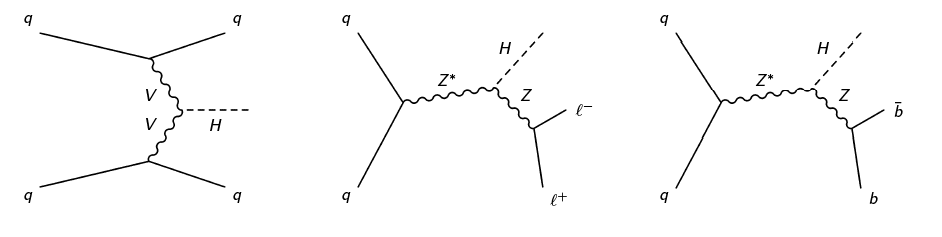
\includegraphics[width=\textwidth]{TalkPics/invcomb021213/feyndiags}
  %% \begin{fmfgraph*}(100,70)
  %%         \fmfleft{i1,i2}
  %%         \fmfright{o1,o2,o3}
  %%         \fmf{fermion}{i1,v1,o1}
  %%         \fmf{fermion}{i2,v2,o3}
  %%         \fmf{phantom,tension=4/5}{v1,v2}
  %%         \fmffreeze
  %%         \fmf{photon,label=$W,,Z$}{v1,v3}
  %%         \fmf{photon,label=$W,,Z$}{v2,v3}
  %%         \fmf{dashes}{v3,o2}
  %%         \fmflabel{$q$}{i1}
  %%         \fmflabel{$q$}{i2}
  %%         \fmflabel{$q$}{o1}
  %%         \fmflabel{$q$}{o3}
  %%         \fmflabel{$H$}{o2}

  %%       \end{fmfgraph*}
}
\date{}
\begin{document}
\begin{fmffile}{studseminarfeynmandiags}

  %TITLE PAGE
  \section{Title}
  \begin{frame}
    \titlepage
    
  \end{frame}

  \begin{frame}
    \frametitle{CMS and the LHC}
    \begin{center}
      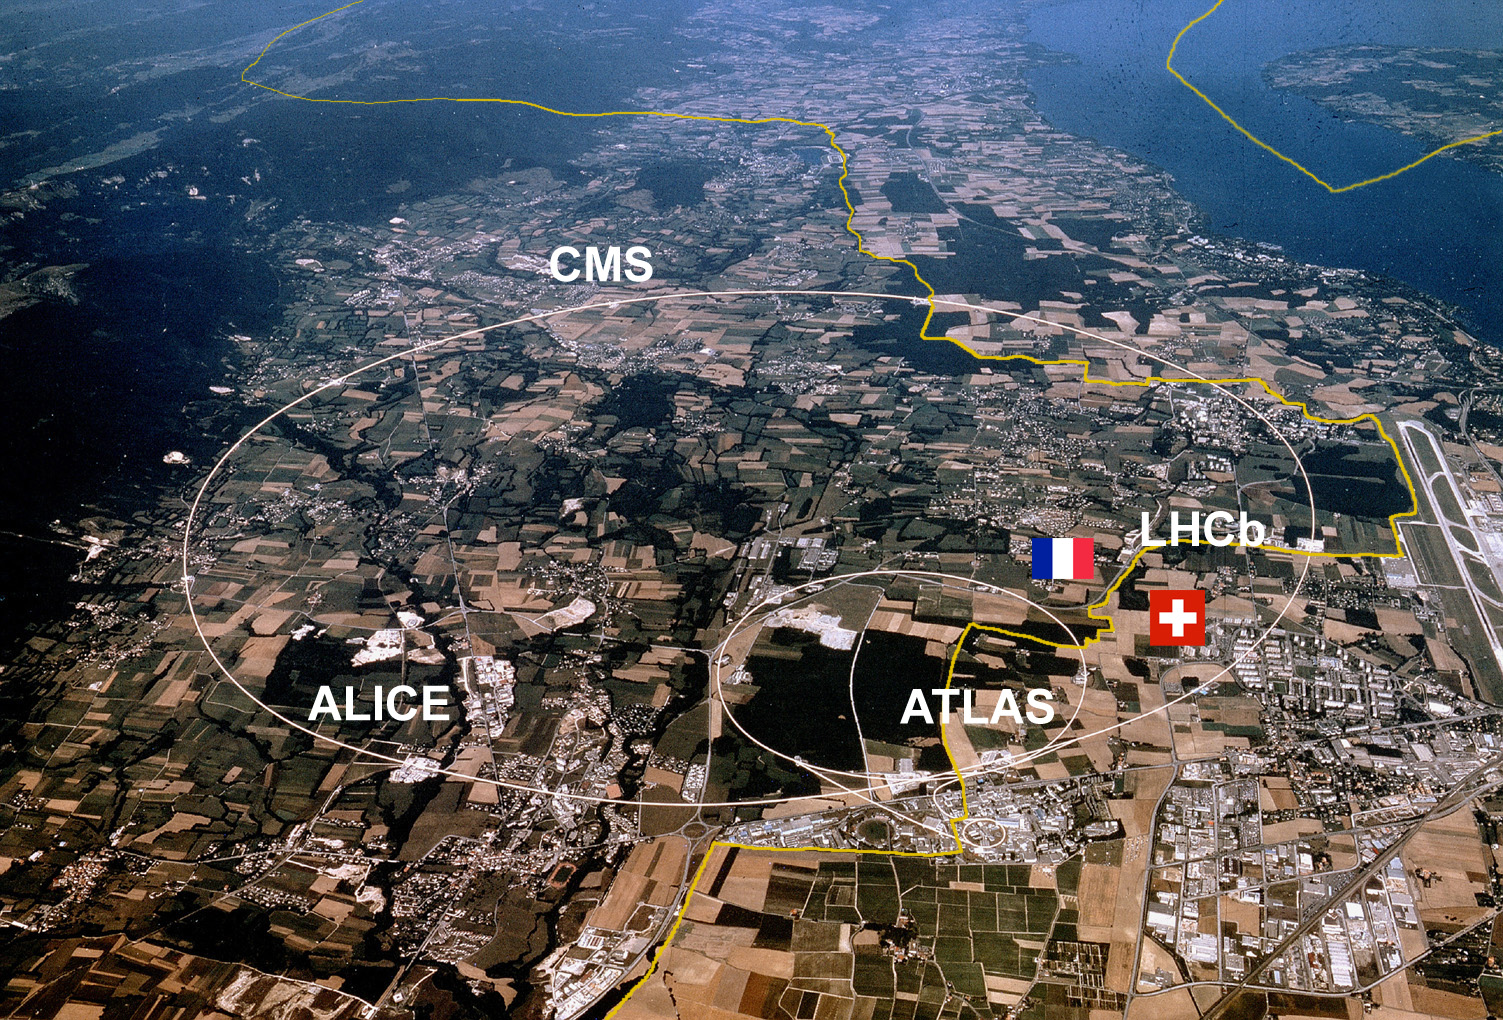
\includegraphics[width=.9\textwidth]{TalkPics/cern-lhc-aerial.jpg}
      \end{center}
  \end{frame}

  \begin{frame}
    \frametitle{CMS}
    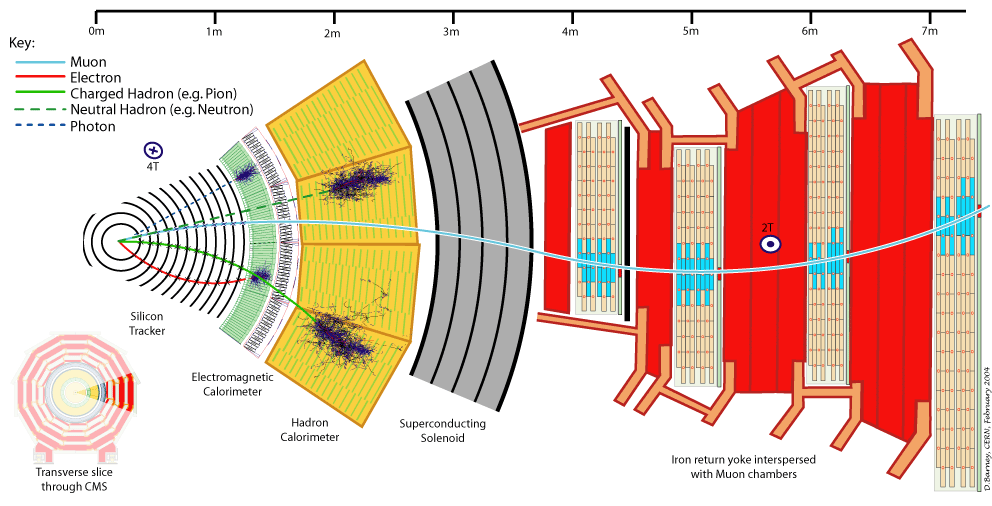
\includegraphics[width=\textwidth]{TalkPics/CMS_Slice.png}
  \end{frame}
  
  %HIGGS BACKGROUND
  \begin{frame}
    \frametitle{The Higgs Boson}
    \begin{columns}
      \column{.5\textwidth}
      \includegraphics[width=\textwidth]{../../Reports/Firstyearreport/XSBR_8TeV_SM.pdf}


      \column{.5\textwidth}
      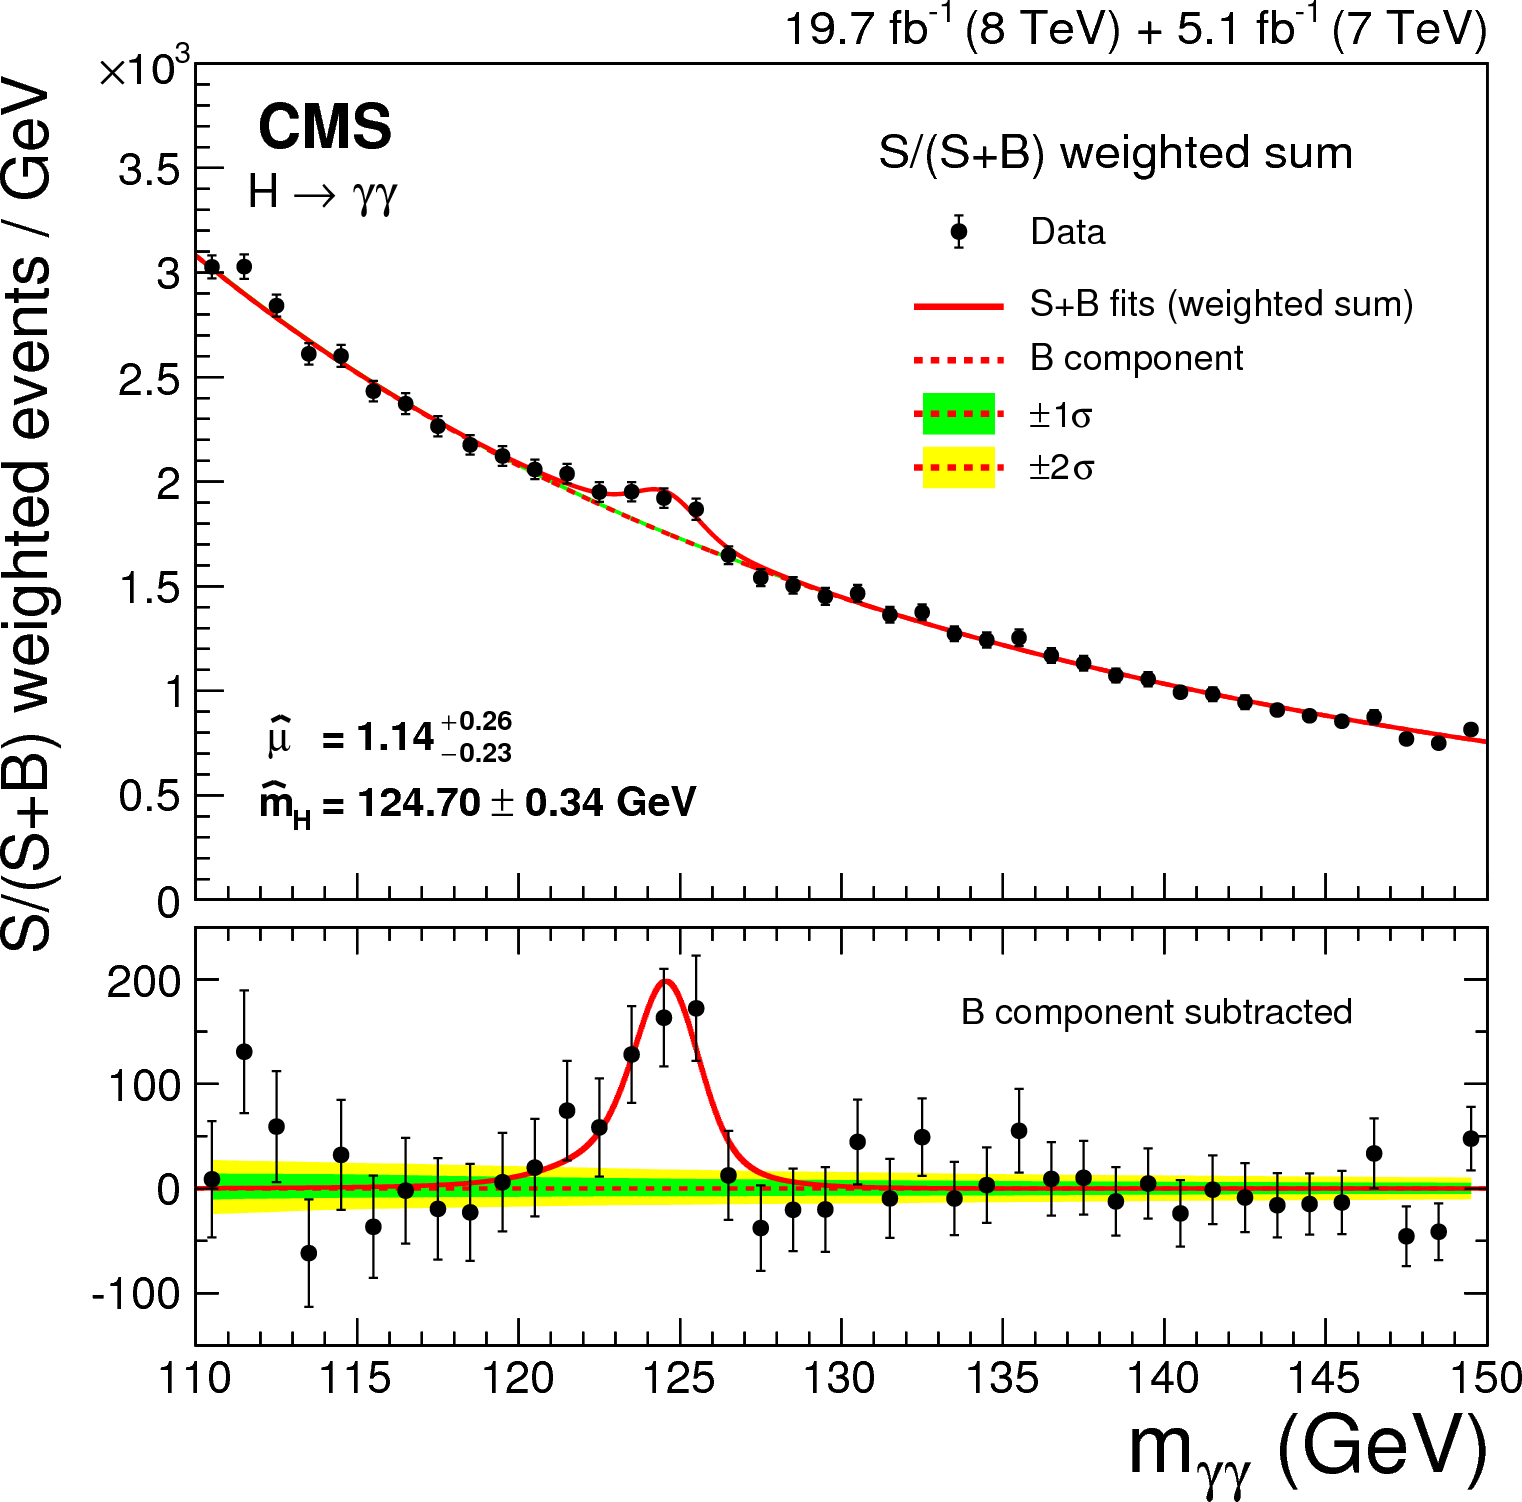
\includegraphics[width=\textwidth]{TalkPics/hgg.png}      

    \end{columns}
  \end{frame}

  \begin{frame}
    \frametitle{Why Higgs to Invisible?}
    \centering
    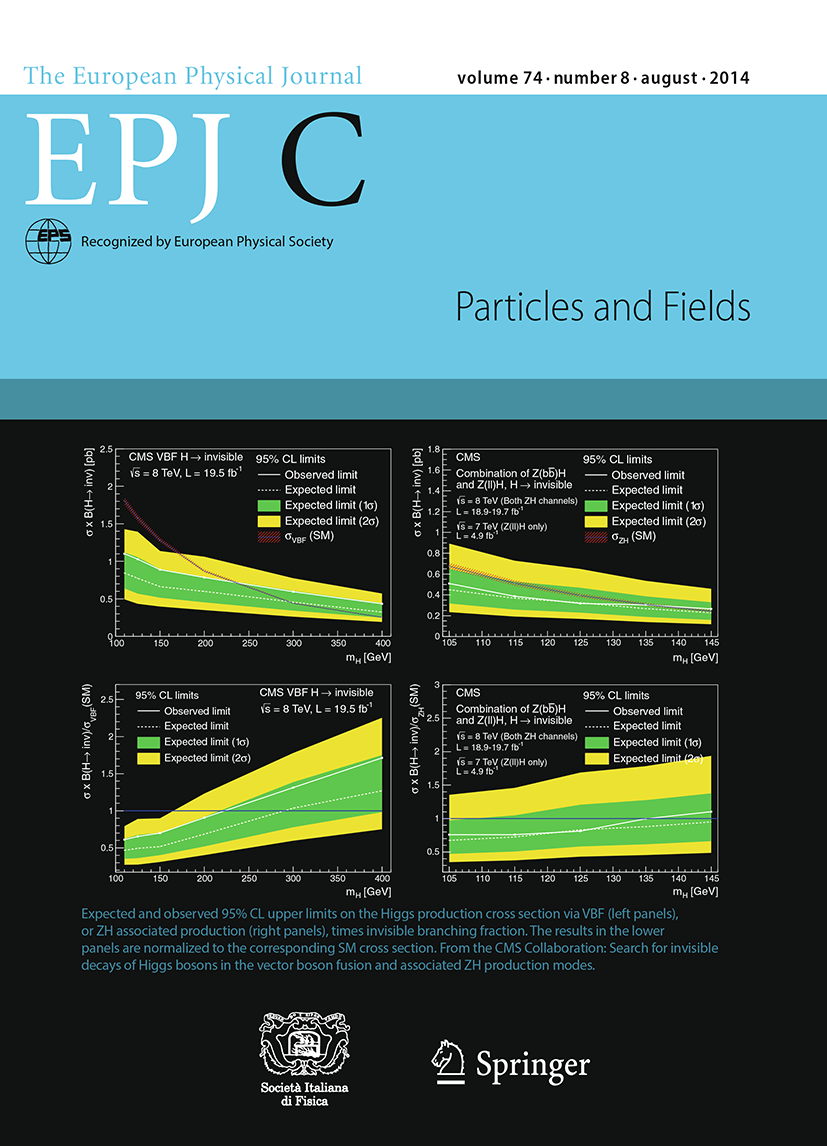
\includegraphics[height=.85\textheight]{TalkPics/EPJCAug2014Cover.png}
  \end{frame}

  \begin{frame}
    \frametitle{Why Higgs to Invisible?}
    \vspace{-.2cm}
    \begin{columns}
      \column{.5\textwidth}
      \begin{block}{\scriptsize Experimental motivation}
        \scriptsize
        \begin{itemize}
        \item At the end of run 1 significant BSM Higgs properties are not excluded:
        \item[-] Limit from ATLAS+CMS on BR$_{BSM}\sim 35\%$
        \end{itemize}
      \end{block}
      \begin{block}{\scriptsize Theoretical motivation}
        \scriptsize
        \begin{itemize}
        \item Many BSM theories predict Higgs boson decays to invisible final states:
        \item[-] e.g. SUSY, extra dimensions, fourth-generation neutrinos
        \item These final state particles are often dark matter candidates
        \end{itemize}
      \end{block}
      \column{.45\textwidth}
      \hfill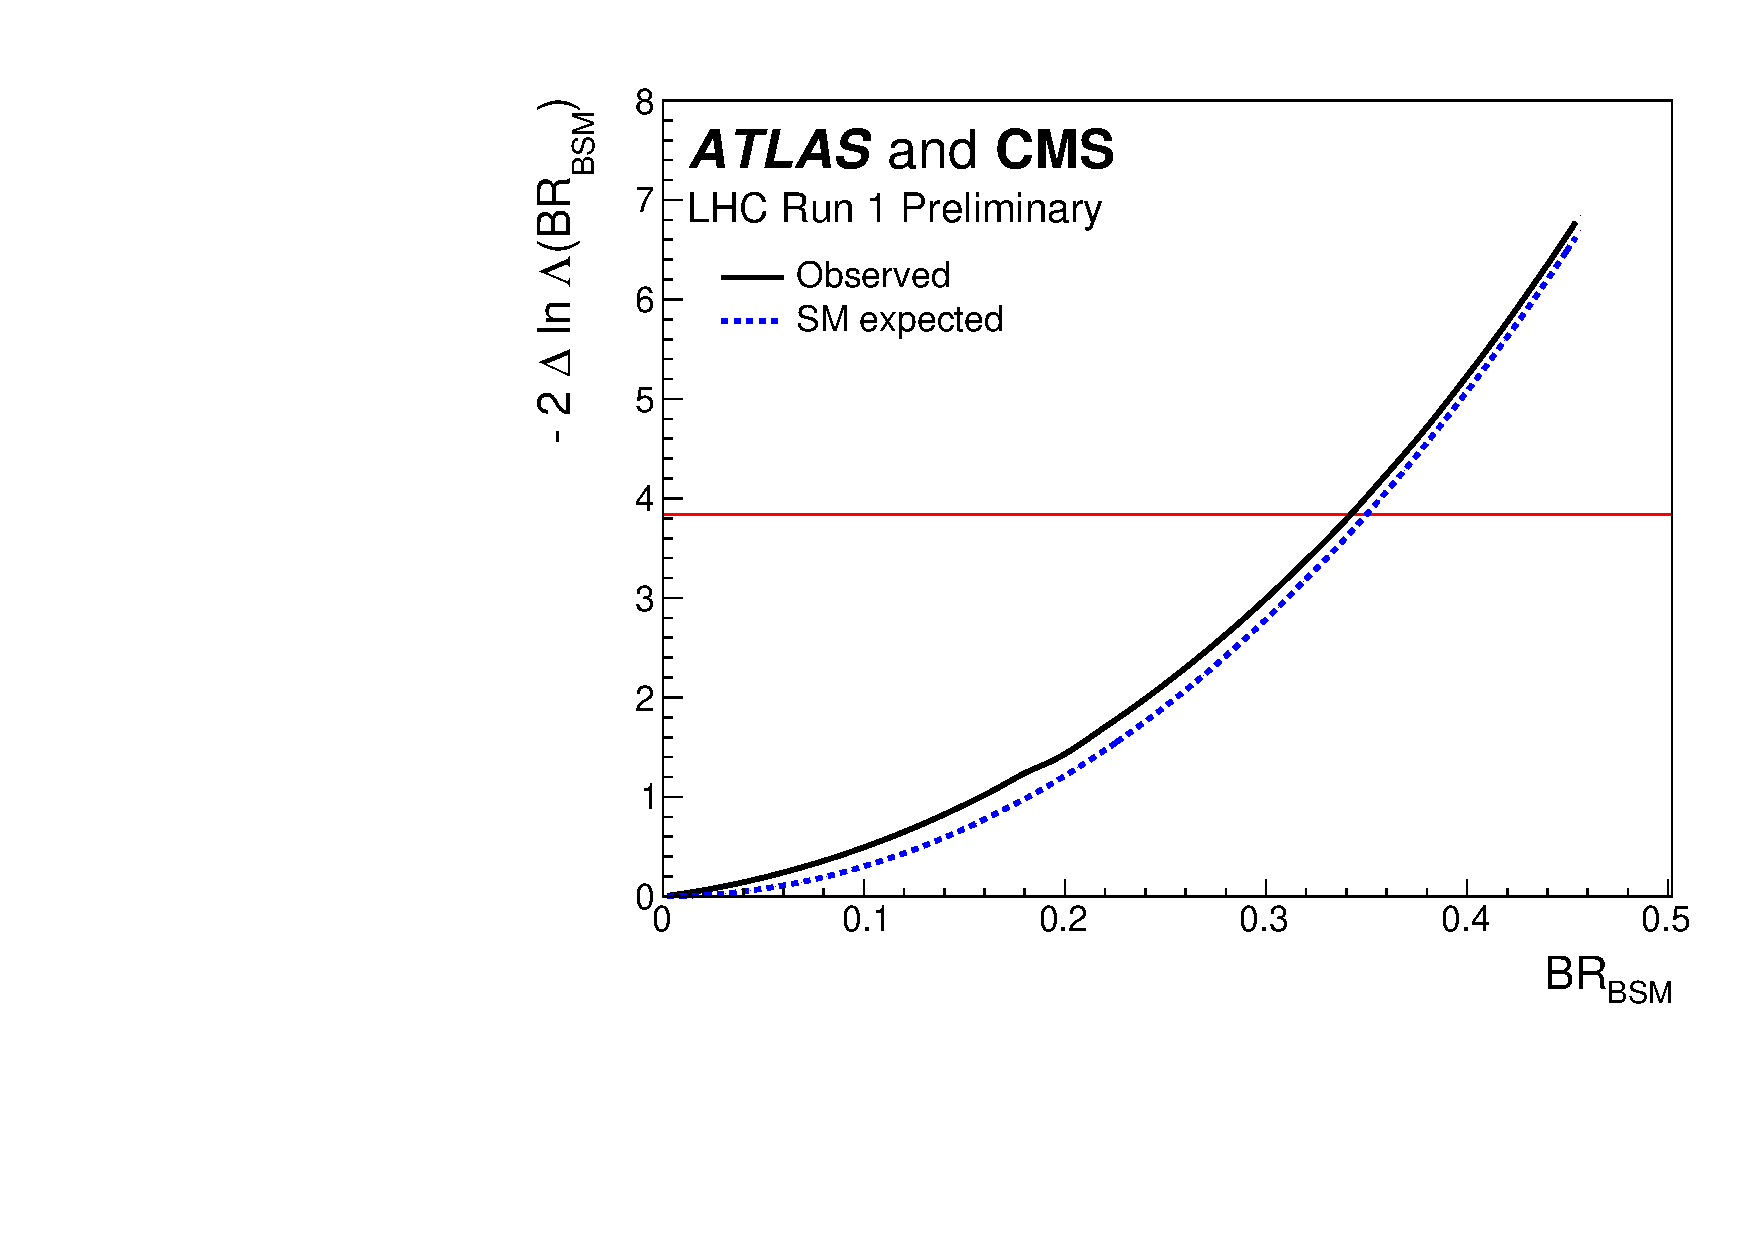
\includegraphics[height=.55\textheight]{TalkPics/iccms300915/CMS-PAS-HIG-15-002_Figure_015.pdf}
      \column{.05\textwidth}
      \begin{turn}{-90}\scriptsize CMS-PAS-HIG-14-009\end{turn}
    \end{columns}
    \begin{columns}
      \column{1.095\textwidth}
    \end{columns}

  \end{frame}

  \begin{frame}
    \frametitle{Direct and Indirect Searches}

    \begin{columns}
      \column{.5\textwidth}
      \vspace{-.8cm}
      \begin{block}{\scriptsize Indirect searches}
        \begin{itemize}
          \scriptsize
        \item BSM Higgs decays affect the total Higgs width:
        \item Visible decays can, therefore, constrain the invisible branching fraction
        \end{itemize}
      \end{block}
      \begin{block}{\scriptsize Direct searches}
        \scriptsize
        \begin{itemize}
        \item Direct searches must be performed in channels where the Higgs recoils against a visible system
        \item We look in the VBF, W/ZH and ggH channels
        \end{itemize}
      \end{block}
      \column{.5\textwidth}

      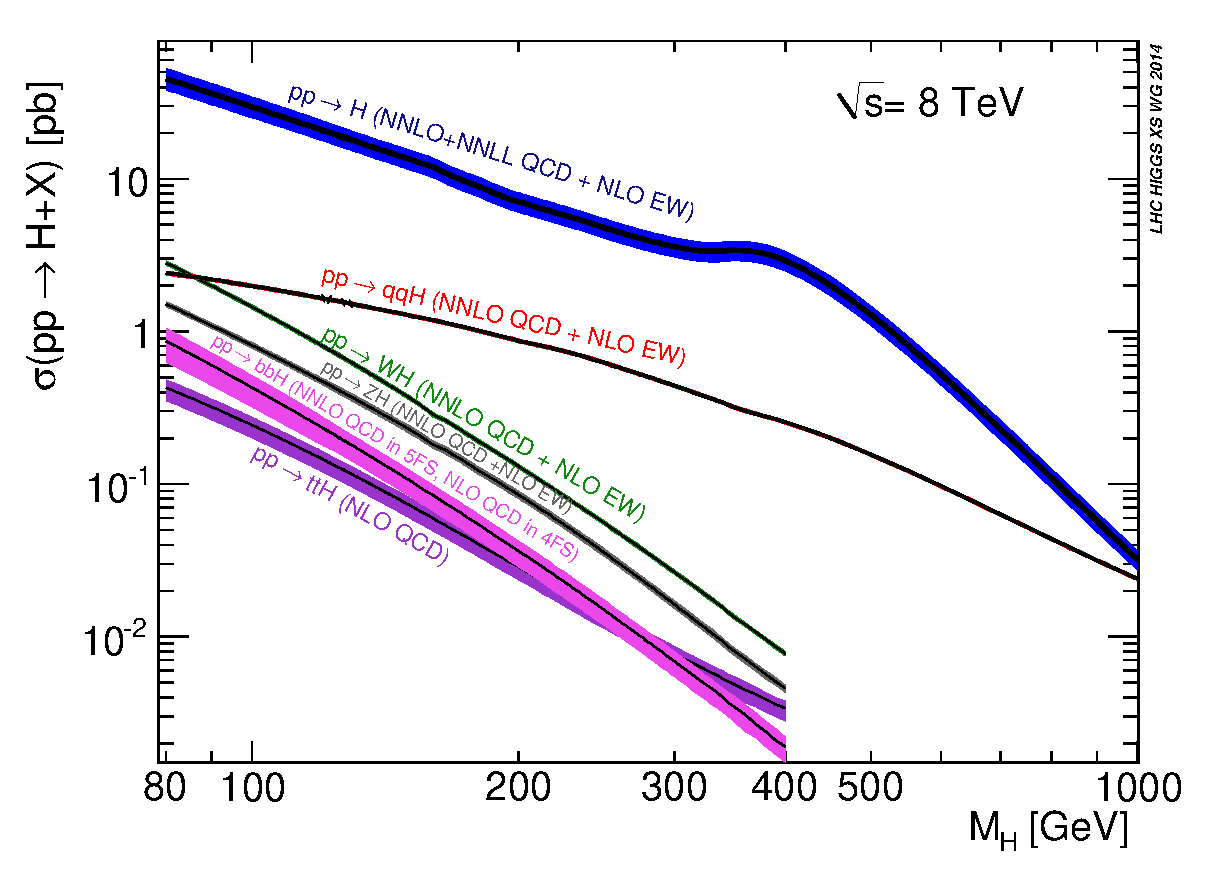
\includegraphics[width=.8\textwidth]{TalkPics/studentseminar221015/XS_8TeV.eps}
      \centering

      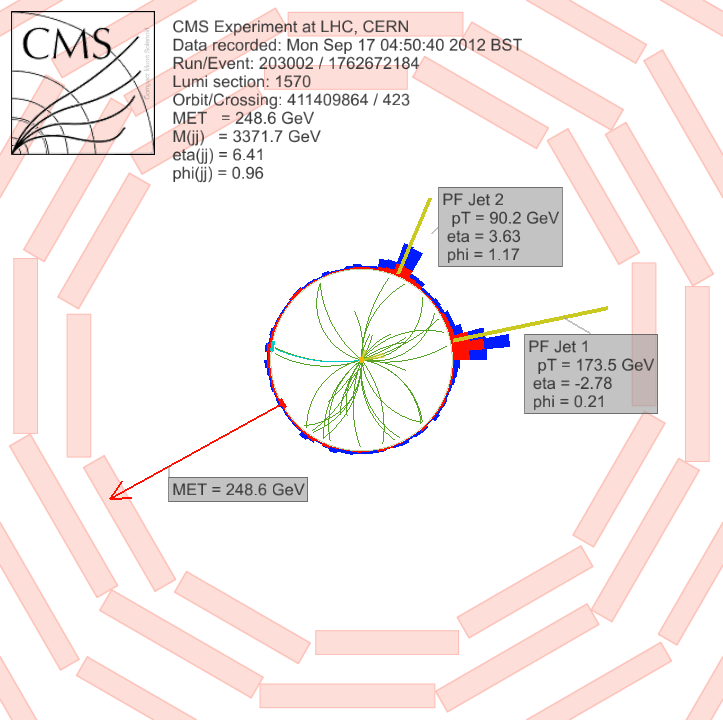
\includegraphics[width=.7\textwidth]{TalkPics/sgs120315/vbfevent.png}
    \end{columns}
  \end{frame}

  \begin{frame}
    \frametitle{VBF outline}
      \begin{block}{\scriptsize Signal Topology and Selection}
        \scriptsize
        \begin{itemize}
        \item Two high $p_{T}$ VBF jets with large rapidity separation
        \item[-] no activity between jets
        \item Large missing transverse momentum (MET)
        \item[-] Cut hard to remove backgrounds
        \end{itemize}
      \end{block}
    \begin{columns}
      \column{.44\textwidth}
      \centering
      \begin{fmfgraph*}(80,60)
        \fmfleft{i1,i2}
        \fmfright{o1,o2,o3}
        \fmf{fermion}{i1,v1,o1}
        \fmf{fermion}{i2,v2,o3}
        \fmf{photon,label=$W,,Z$,l.side=left}{v1,v4}
        \fmf{photon}{v4,v3}
        \fmf{photon,label=$W,,Z$,l.side=right}{v2,v5}
        \fmf{photon}{v5,v3}
        \fmf{dashes}{v3,v6}
        \fmf{dashes}{v6,o2}
        \fmflabel{$q$}{i1}
        \fmflabel{$q$}{i2}
        \fmflabel{$q$}{o1}
        \fmflabel{$q$}{o3}
        \fmflabel{$H$}{o2}
      \end{fmfgraph*}
      \vspace{.5cm}
      \column{.5\textwidth}
        \hfill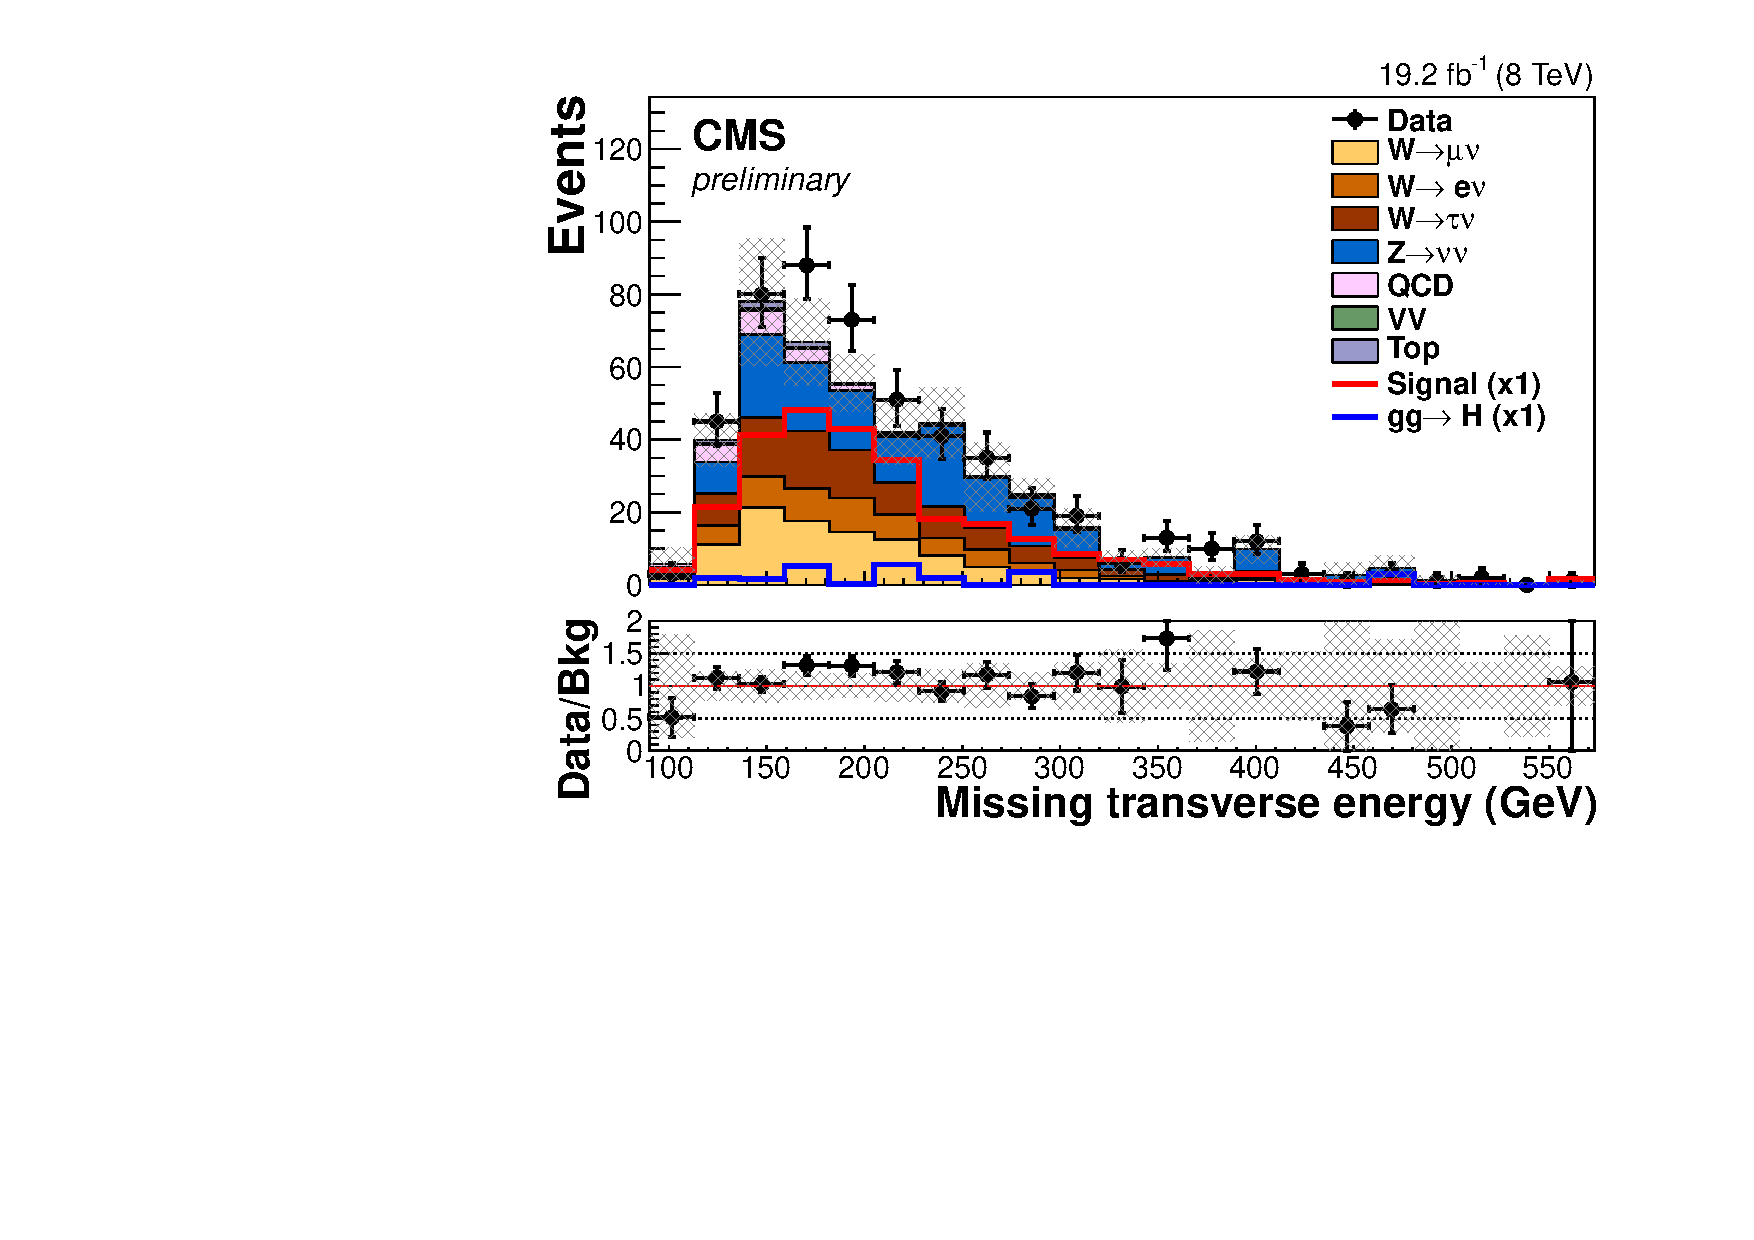
\includegraphics[height=.55\textheight]{TalkPics/studentseminar221015/vbfmet.pdf}
    \end{columns}
  \end{frame}

  \begin{frame}
    \frametitle{Backgrounds}
    %WJETS
    \begin{columns}
      \column{.33\textwidth}
      \begin{block}{W+jets}
        \centering
        \begin{fmfgraph*}(60,50)
          \fmftop{i1,m1,m2,o1}
          \fmfbottom{i2,o2}
          \fmf{fermion,label=$e/\mu/\tau$,label.side=left}{v2,m1}
          \fmf{fermion,label=$\nu$,label.side=right}{v2,m2}
          \fmf{photon,tension=7/5,label=$W$}{v1,v2}
          \fmf{fermion}{v1,i2}
          \fmf{fermion}{v1,o2}
          \fmflabel{$jet$}{i2}
          \fmflabel{$jet$}{o2}
        \end{fmfgraph*}
        \vspace{.2cm}
        \begin{itemize}
          \item Veto leptons
        \end{itemize}
      \end{block}

      \column{.33\textwidth}
      \begin{block}{Z+jets}
        \centering
        \begin{fmfgraph*}(60,50)
          \fmftop{i1,m1,m2,o1}
          \fmfbottom{i2,o2}
          \fmf{fermion}{v1,i2}
          \fmf{fermion}{v1,o2}
          \fmf{photon,tension=7/5,label=$Z$}{v1,v2}
          \fmf{fermion,label=$\nu$,label.side=left}{v2,m1}
          \fmf{fermion,label=$\nu$,label.side=right}{v2,m2}
          \fmflabel{$jet$}{i2}
          \fmflabel{$jet$}{o2}
        \end{fmfgraph*}
        \vspace{.2cm}
        \begin{itemize}
          \item Irreducible
        \end{itemize}
      \end{block}

      \column{.33\textwidth}
      \begin{block}{QCD - multijet}
        \centering
        \begin{fmfgraph*}(60,50)
          \fmftop{i1,m1,m2,m3,m4,o1}
          \fmfbottom{i2,o2}
          \fmf{fermion,tension=4}{v1,i2}
          \fmf{fermion,tension=4}{v1,o2}
          \fmf{fermion,label=$jets$,label.side=left}{v1,m1}
          \fmf{dashes}{v1,m3}
          \fmflabel{$jet$}{i2}
          \fmflabel{$jet$}{o2}
        \end{fmfgraph*}
        \vspace{.2cm}
      \begin{itemize}
      \item See next slide
      \end{itemize}
      \end{block}
    \end{columns}
  \end{frame}

  \begin{frame}
    \frametitle{Reducing QCD Backgrounds}
    %WJETS
      \begin{block}{MET significance}
        \centering
        \begin{fmfgraph*}(60,50)
          \fmftop{i1,m1,m2,m3,m4,m5,m6,m7,o1}
          \fmfbottom{i2,m8,m9,m10,m11,o2}
          \fmf{fermion,tension=4}{v1,i2}
          \fmf{fermion,tension=4}{v1,o2}
          \fmf{fermion,label=$jets$,label.side=left}{v1,m1}
          \fmf{dashes}{v1,m3}
          \fmf{fermion}{v1,m4}
          \fmf{fermion}{v1,m5}
          \fmf{fermion}{v1,m6}
          \fmf{fermion}{v1,m7}
          \fmf{fermion}{v1,m8}
          \fmf{fermion}{v1,m9}
          \fmf{fermion}{v1,m10}
          \fmf{fermion}{v1,m11}
          \fmflabel{$jet$}{i2}
          \fmflabel{$jet$}{o2}
        \end{fmfgraph*}
        \hspace{1.5cm}
        VS
        \hspace{1.5cm}
        \begin{fmfgraph*}(60,50)
          \fmftop{i1,m1,m2,m3,m4,m5,m6,m7,o1}
          \fmfbottom{i2,m8,m9,m10,m11,o2}
          \fmf{fermion,tension=4}{v1,i2}
          \fmf{fermion,tension=4}{v1,o2}
          \fmf{fermion,label=$jets$,label.side=left}{v1,m1}
          \fmf{dashes}{v1,m3}
          \fmflabel{$jet$}{i2}
          \fmflabel{$jet$}{o2}
        \end{fmfgraph*}


        \vspace{.2cm}
      \end{block}

      \begin{block}{min$\Delta\phi$(j,MET)}
        \centering
        \begin{fmfgraph*}(60,50)
          \fmftop{i1,m1,m2,m3,m4,m5,m6,m7o1}
          \fmfbottom{i2,o2}
          \fmf{fermion,tension=4}{v1,i2}
          \fmf{fermion,tension=4}{v1,o2}
          \fmf{fermion,label=$jets$,label.side=left}{v1,m1}
          \fmf{dashes}{v1,m2}
          \fmflabel{$jet$}{i2}
          \fmflabel{$jet$}{o2}
        \end{fmfgraph*}
        \vspace{.2cm}
      \end{block}

  \end{frame}
  
  \begin{frame}
    \frametitle{Background estimation}
      \vspace{-.3cm}
      \begin{block}{\footnotesize Data Driven Background Estimation}
        \scriptsize
        \begin{itemize}
          \item Choose control region enriched in background
          \item Use MC signal-control ratio to go to signal region:
          $N^{signal}_{Bkg} = (N^{control}_{obs}-N^{control}_{other bkgs}) \cdot \frac{N^{signal}_{MC}}{N^{control}_{MC}}.$
        \end{itemize}
      \end{block}
    \begin{tikzpicture}
      \node[anchor=south west,inner sep=0] (image) at (0,0) { \begin{columns}\column{.5\textwidth}      \begin{block}{\scriptsize Control Region: Single Muon} 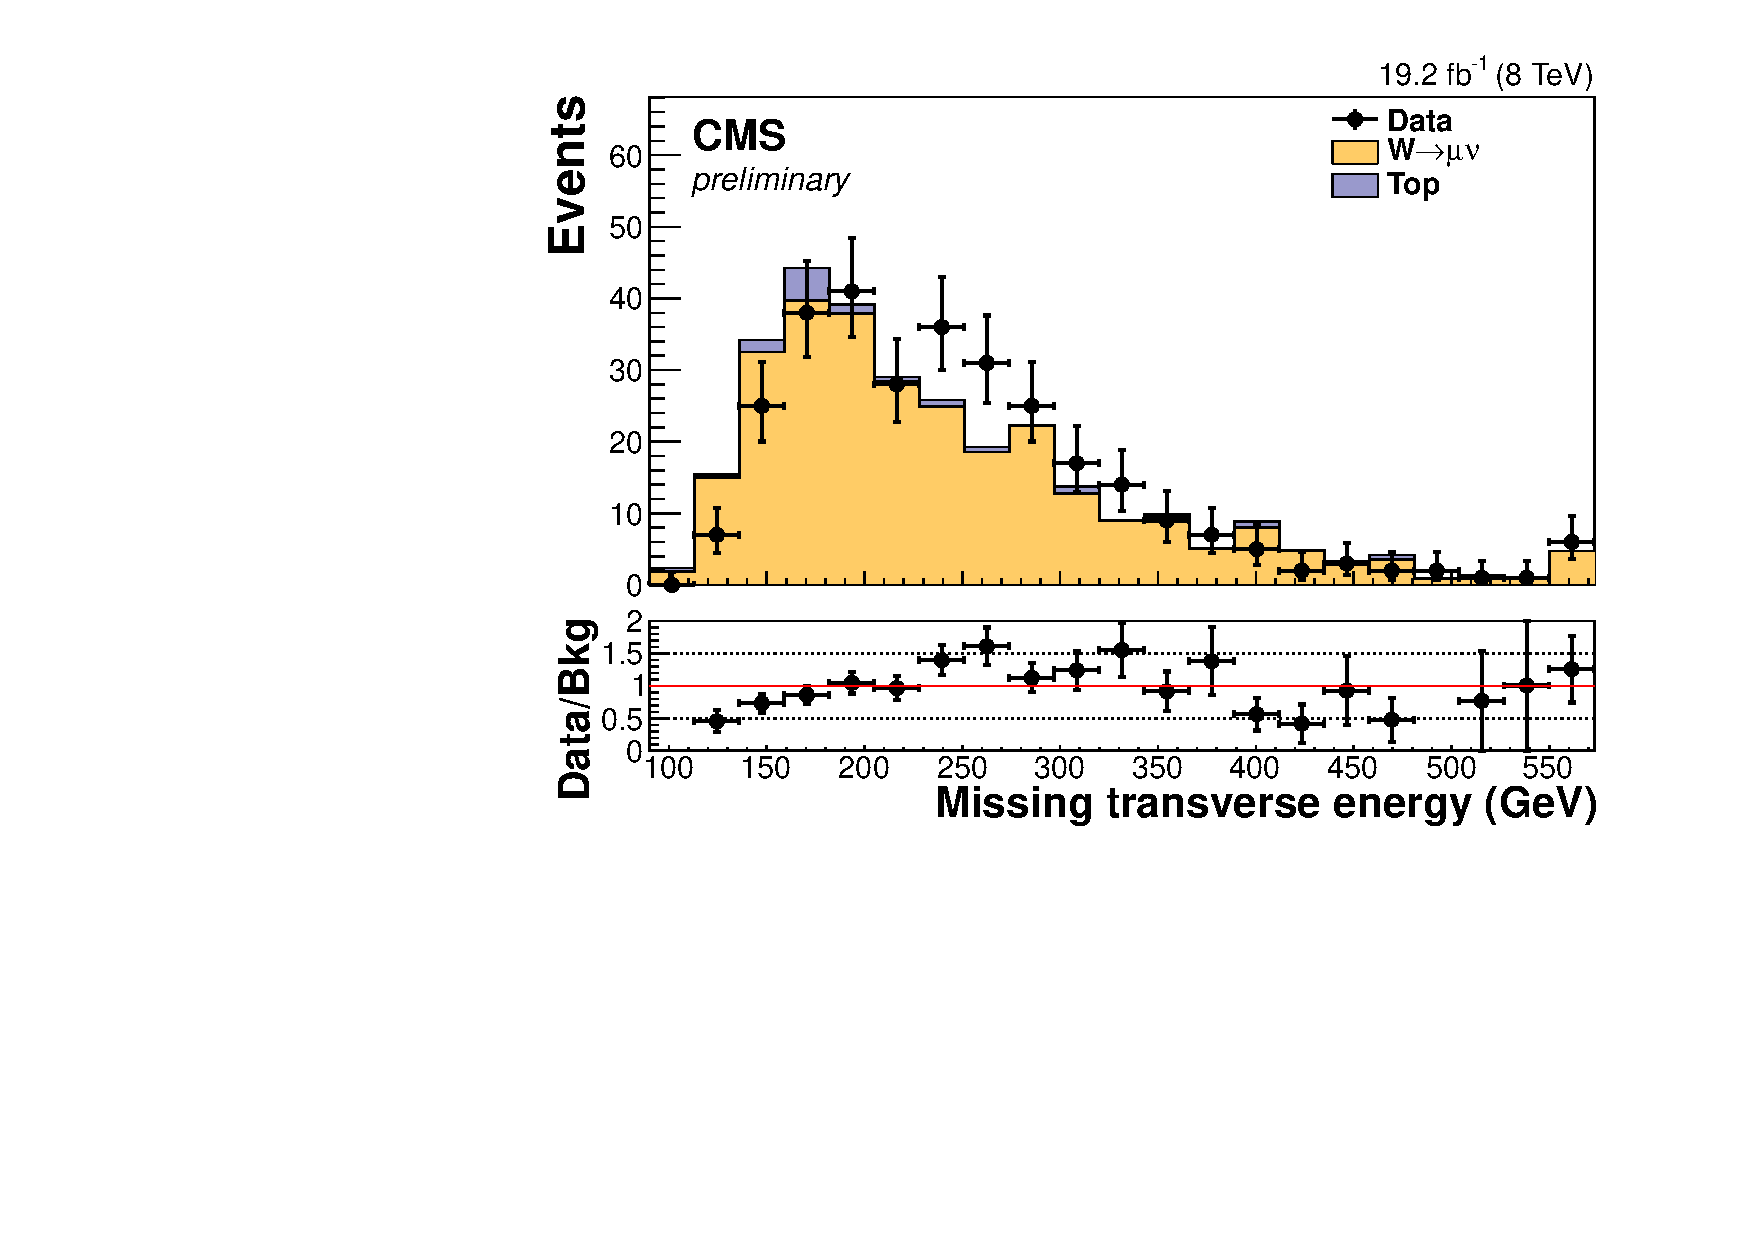
\includegraphics[width=\textwidth]{TalkPics/studentseminar221015/hig14038figures/output_sigreg/munu_metnomuons.pdf} \end{block}
    \column{.5\textwidth} \begin{block}{\scriptsize Signal Region: Lepton veto}  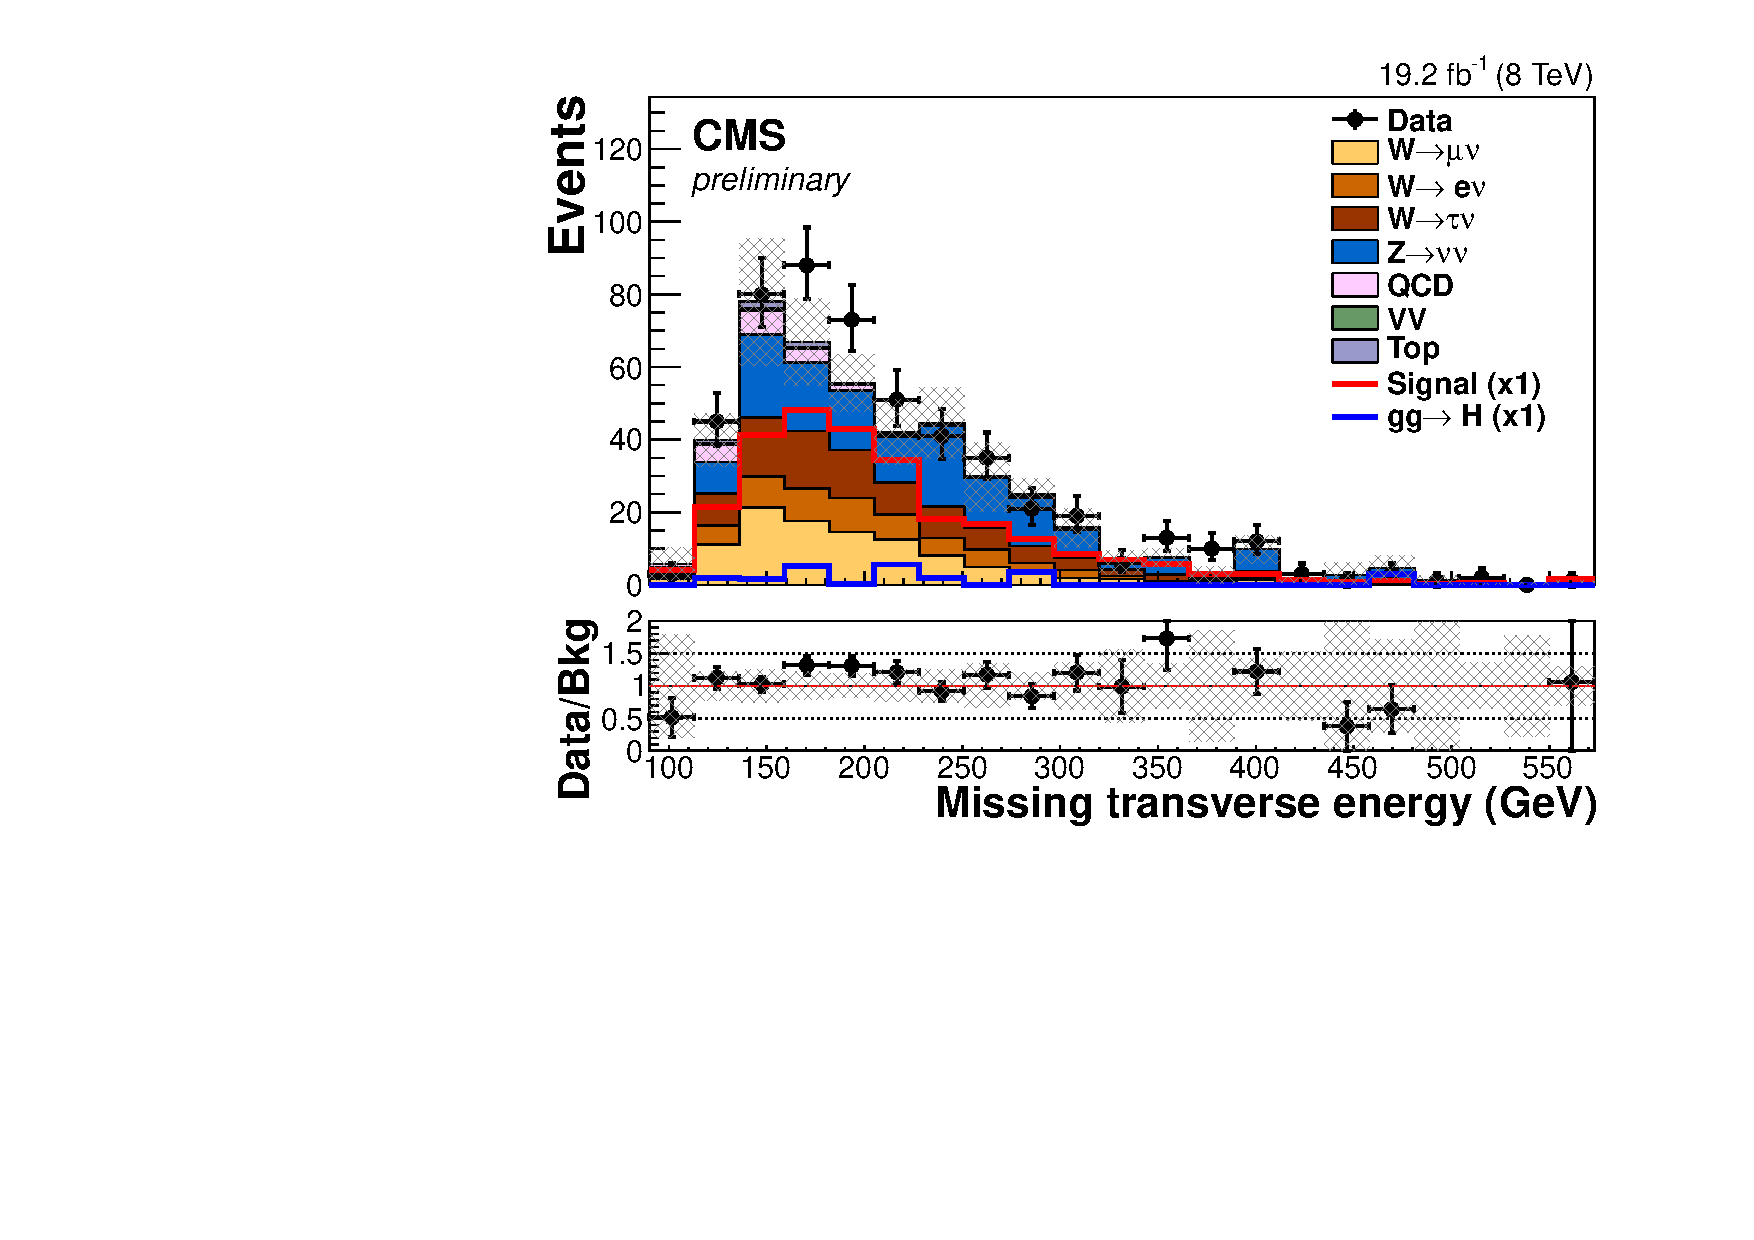
\includegraphics[width=\textwidth]{TalkPics/studentseminar221015/hig14038figures/output_sigreg/nunu_metnomuons.pdf} \end{block} \end{columns} };
      \begin{scope}[x={(image.south east)},y={(image.north west)}]
        \path[->,color=red,ultra thick] (0.3,0.5) edge (0.6,0.5);
      \end{scope}
    \end{tikzpicture}

      %!!background control region plots

    
  \end{frame}
  \begin{frame}
    \frametitle{VBF results}
%!!Replace with hig-14-038
      \scriptsize
      \begin{tikzpicture}
        \draw node[text width=\textwidth, anchor=south west,inner sep=0] (image) at (0,0) {
          \begin{block}{}
          \begin{itemize}
           \item Number of events within one $\sigma$ of the SM expectation:
            \begin{tabular}{lc}
              \hline
              Total background & $439.7\pm 41.0 (stat.) \pm 55.8 (syst.)$ \\
              \hline
              VBF H(inv.) assuming B(H$\rightarrow$inv)=100\% &  $273.4 \pm 31.2(syst.)$ \\
              ggF H(inv.) assuming B(H$\rightarrow$inv)=100\%& $22.6 \pm 15.6 (syst.)$ \\
              \hline
              Observed data & 508 \\
              \hline
            \end{tabular}
            
          \item Set limits on $\sigma$x$B(H\rightarrow inv)$
          \item[-] Perform a single bin counting experiment using $CL_{S}$ method
          \item[-] Observed(expected) 95\% C.L. limit on $B(H\rightarrow inv)$ is 0.57 (0.40)
          \end{itemize}
          \end{block}
          
        };
      \node(comment)[below of=image,anchor=south,inner sep=0,node distance=4cm,visible on=<2>] {
        \huge \textcolor{red}{What does this mean?}
      };

      \begin{scope}[x={(image.south east)},y={(image.north west)}]
        \path[->,color=red,ultra thick,visible on=<2>] (comment.north) edge (0.65,0.17);
      \end{scope}[x={(image.south east)},y={(image.north west)}]
      \end{tikzpicture}

  \end{frame}

  \begin{frame}
    \frametitle{CLs}
    \scriptsize
    \begin{block}{}
      \begin{itemize}
      \item Want to exclude signal models which are less than 5\% likely to give data
      \item Exclude everything where shaded area (CL$_{S+B}$)  is $<5\%$
      \end{itemize}
    \end{block}
    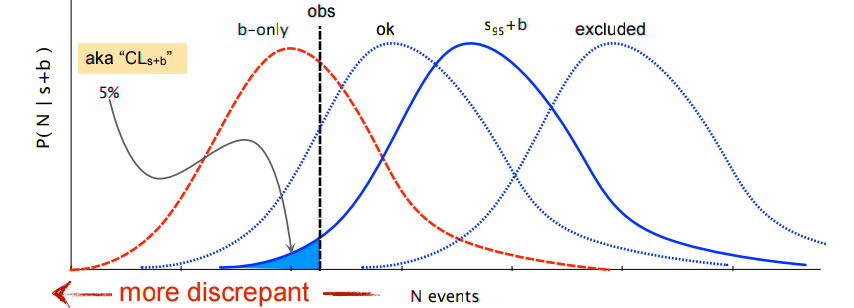
\includegraphics[width=\textwidth]{TalkPics/studentseminar221015/clsplusb.png}
  \end{frame}

  \begin{frame}
    \frametitle{CLs}
    \scriptsize
    \begin{block}{}
      \begin{itemize}
      \item What if background only model is also unlikely?
      \item What if you have no sensitivity even to the background?
      \item Risk of overexcluding
      \end{itemize}
    \end{block}
    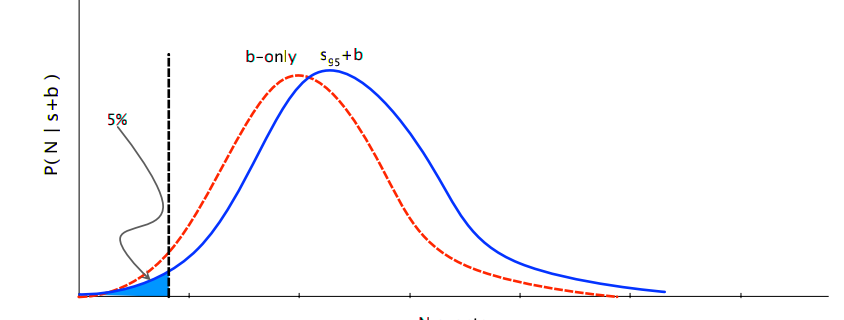
\includegraphics[width=\textwidth]{TalkPics/studentseminar221015/cls1.png}
  \end{frame}

  \begin{frame}
    \frametitle{CLs}
    \scriptsize
    \begin{block}{}
      \begin{itemize}
      \item $CL_{S}=\frac{CL_{S+B}}{CL_{B}}$
      \item Gets bigger if $CL_{B}$ is small too
      \item Avoids overexcluding
      \end{itemize}
    \end{block}
    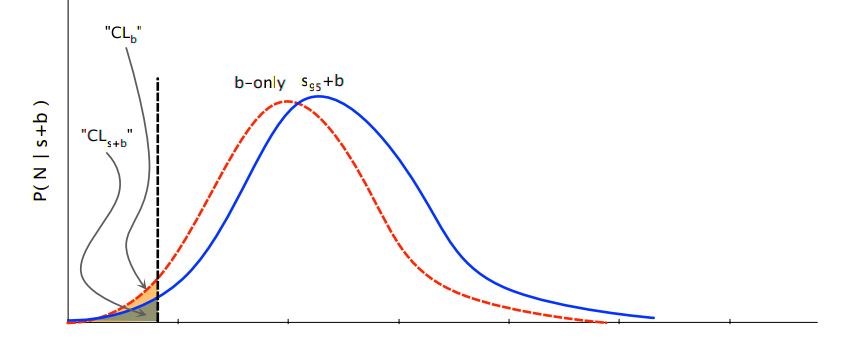
\includegraphics[width=\textwidth]{TalkPics/studentseminar221015/cls2.png}
  \end{frame}


  \begin{frame}
    \frametitle{Combinations}
    %!!what do you need to worry about with combinations
  \end{frame}

  \begin{frame}
    \frametitle{Combination Results}
    \begin{block}{}
      \scriptsize
      \begin{itemize}
      \item The individual limits on $\sigma$x$B(H\rightarrow inv)$ from all channels are combined
      \item[-] SM production cross-sections are used to interpret this as a limit on B(H$\rightarrow$inv)
      \end{itemize}
    \end{block}
    \begin{columns}
      \column{.65\textwidth}
      \centering
      \begin{columns}
        \column{.95\textwidth}
      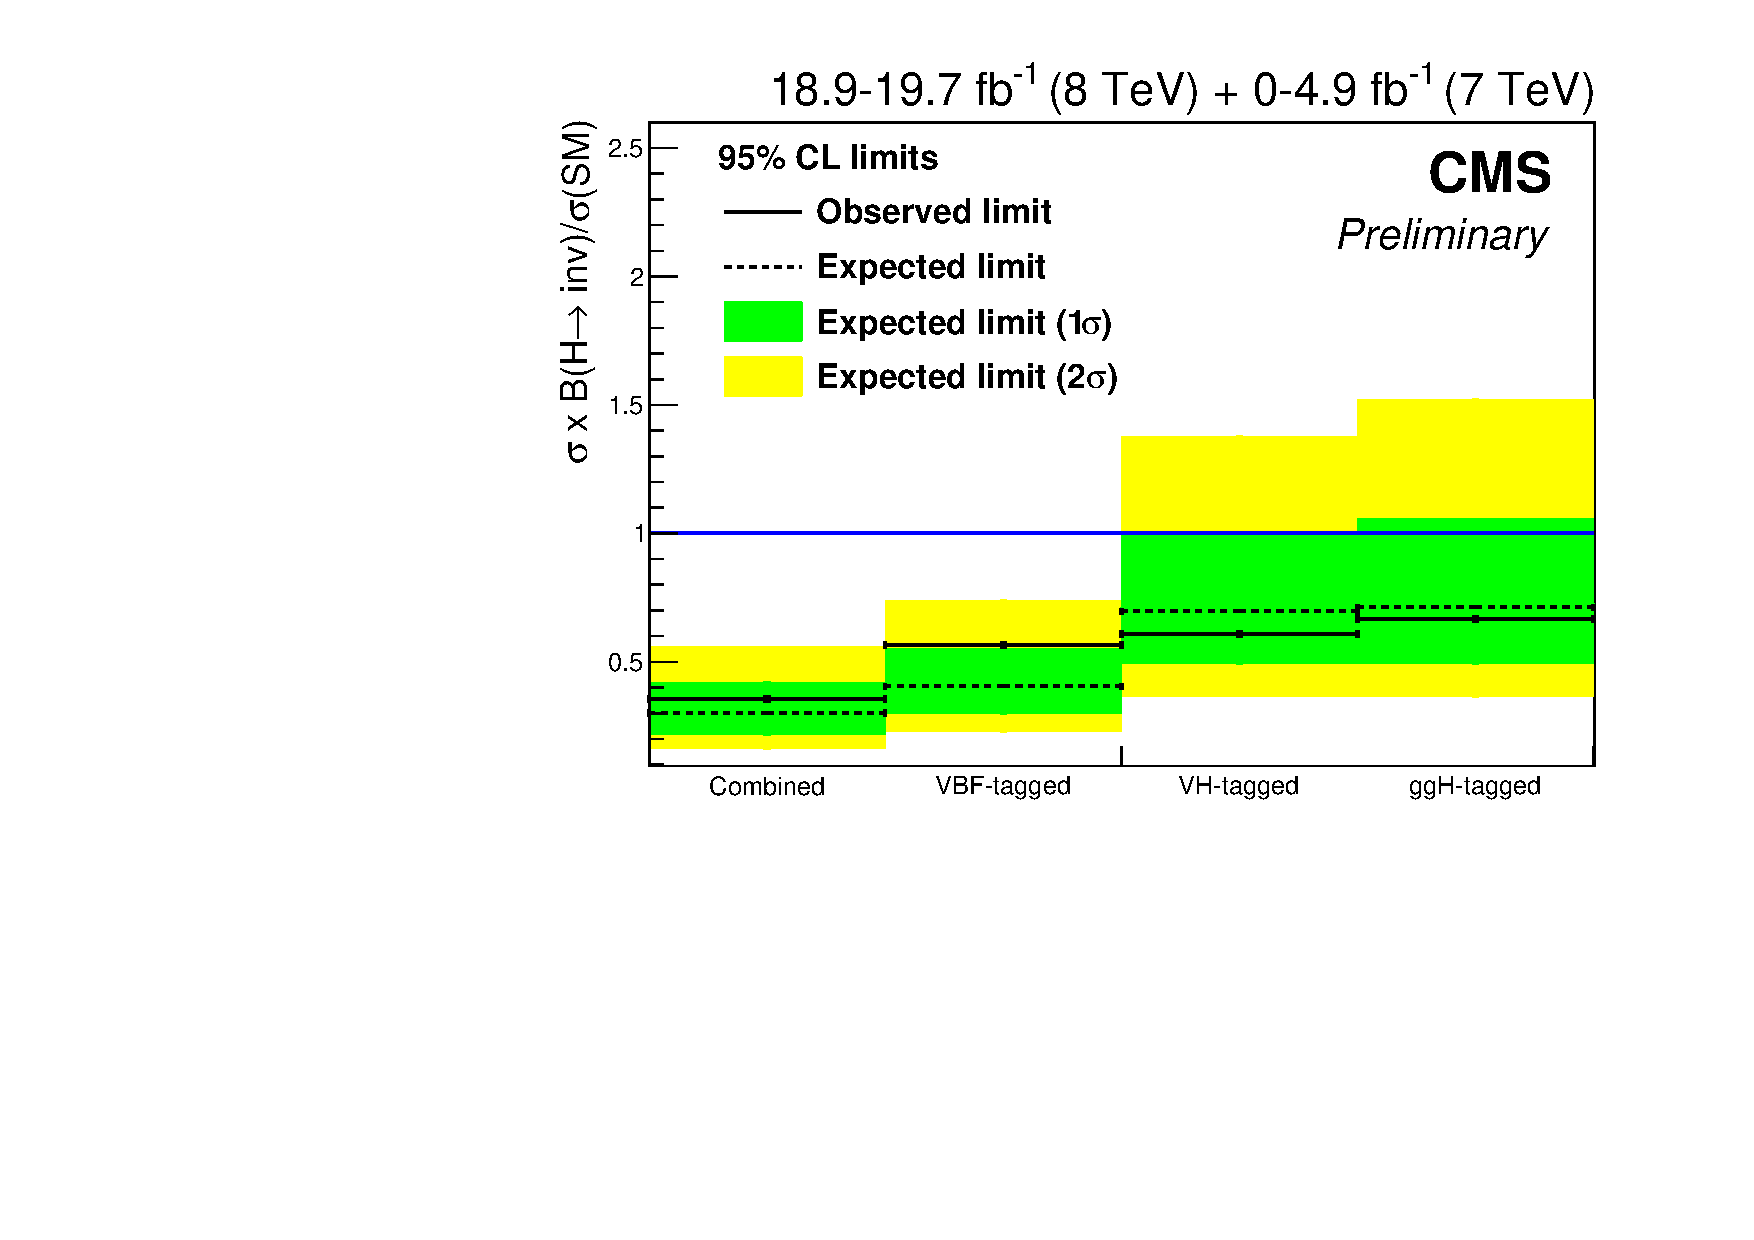
\includegraphics[clip=true,trim=0 0 0 0, width=1.1\textwidth]{TalkPics/studentseminar221015/hig15012figures/channellimit.pdf}
        \column{.05\textwidth}
      \end{columns}
      \column{.35\textwidth}
      \scriptsize
      \begin{block}{}
        Observed (expected) limits on B(H$\rightarrow$inv) at 95\% C.L. for $m_{H}$=125 GeV

        \centering
        \begin{tabular}{lc}
          \hline
          Channel & Limit/\% \\
          \hline
          VBF-tagged & 57(40) \\
          VH-tagged & 60(69) \\
          ggH-tagged & 67(71) \\
          \hline
          Combined & \textcolor{red}{36(30)} \\
          \hline
        \end{tabular}
      \end{block}
    \end{columns}
  \end{frame}

  \begin{frame}
    \frametitle{Signatures of Dark Matter (DM)}
    \vspace{-.2cm}
    \begin{block}{}
      \scriptsize
      \begin{itemize}
      \item If DM couples to the Higgs the following diagrams are possible
      \end{itemize}
    \end{block}
    \vspace{-.2cm}
    \begin{columns}
      \column{.35\textwidth}
      \begin{block}{\scriptsize Direct Detection - e.g. LUX}
        \vspace{.3cm}
        \begin{fmfgraph*}(100,70)
          \fmfleft{i1,i2}
          \fmfright{o1,o2}
          \fmf{fermion}{i1,v1,o1}
          \fmf{fermion}{i2,v2,o2}
          \fmf{dashes,label=$H$}{v1,v2}
          \fmffreeze
          \fmflabel{$N$}{i1}
          \fmflabel{$\chi$}{i2}
          \fmflabel{$N$}{o1}
          \fmflabel{$\chi$}{o2}
        \end{fmfgraph*}
        \vspace{.3cm}
      \end{block}

      \column{.35\textwidth}
      \begin{block}{\scriptsize Invisible Higgs - LHC}
        \vspace{.3cm}
        \begin{fmfgraph*}(100,70)
          \fmfleft{i1,i2}
          \fmfright{o1,o2}
          \fmf{fermion}{i1,v1,i2}
          \fmf{fermion}{o1,v2,o2}
          \fmf{dashes,label=$H$}{v1,v2}
          \fmffreeze
          %\fmflabel{$f/w/Z$}{i1}
          \fmflabel{$\chi$}{o1}
          %\fmflabel{$f/W/Z$}{i2}
          \fmflabel{$\chi$}{o2}
        \end{fmfgraph*}
        \vspace{.3cm}
      \end{block}
      \column{.35\textwidth}
      \begin{block}{\scriptsize Annihilation - e.g. WMAP}
        \vspace{.3cm}
        \begin{fmfgraph*}(100,70)
          \fmfleft{i1,i2}
          \fmfright{o1,o2}
          \fmf{fermion}{i1,v1,i2}
          \fmf{fermion}{o1,v2,o2}
          \fmf{dashes,label=$H$}{v1,v2}
          \fmffreeze
          %\fmflabel{$f/w/Z$}{i1}
          \fmflabel{$\chi$}{i1}
          %\fmflabel{$f/W/Z$}{i2}
          \fmflabel{$\chi$}{i2}
        \end{fmfgraph*}
        \vspace{.3cm}
      \end{block}
    \end{columns}
    \begin{block}{}
      \scriptsize
      \begin{itemize}
      \item Limits on $\mathcal{B}$(H$\rightarrow$inv) therefore constrain Higgs Portal DM models
      \item[-] These constraints are directly comparable to those from other experiments
      \end{itemize}
    \end{block}
  \end{frame}



  \begin{frame}
    \frametitle{Dark Matter Interpretation}
    \scriptsize
    \vspace{-.3cm}
    \begin{block}{}
      \begin{itemize}
      \item Previously used an effective field theory model which translates B$(H\rightarrow inv)$ into a DM-nucleon cross-section
      \item Consider three DM spin scenarios: scalar, vector, Majorana fermion:
      \item[-] all but one go to infinity as the mass goes to zero
      \end{itemize}
    \end{block}
    \centering
    \begin{tikzpicture}
      \node[anchor=south west,inner sep=0] (image) at (0,0) {    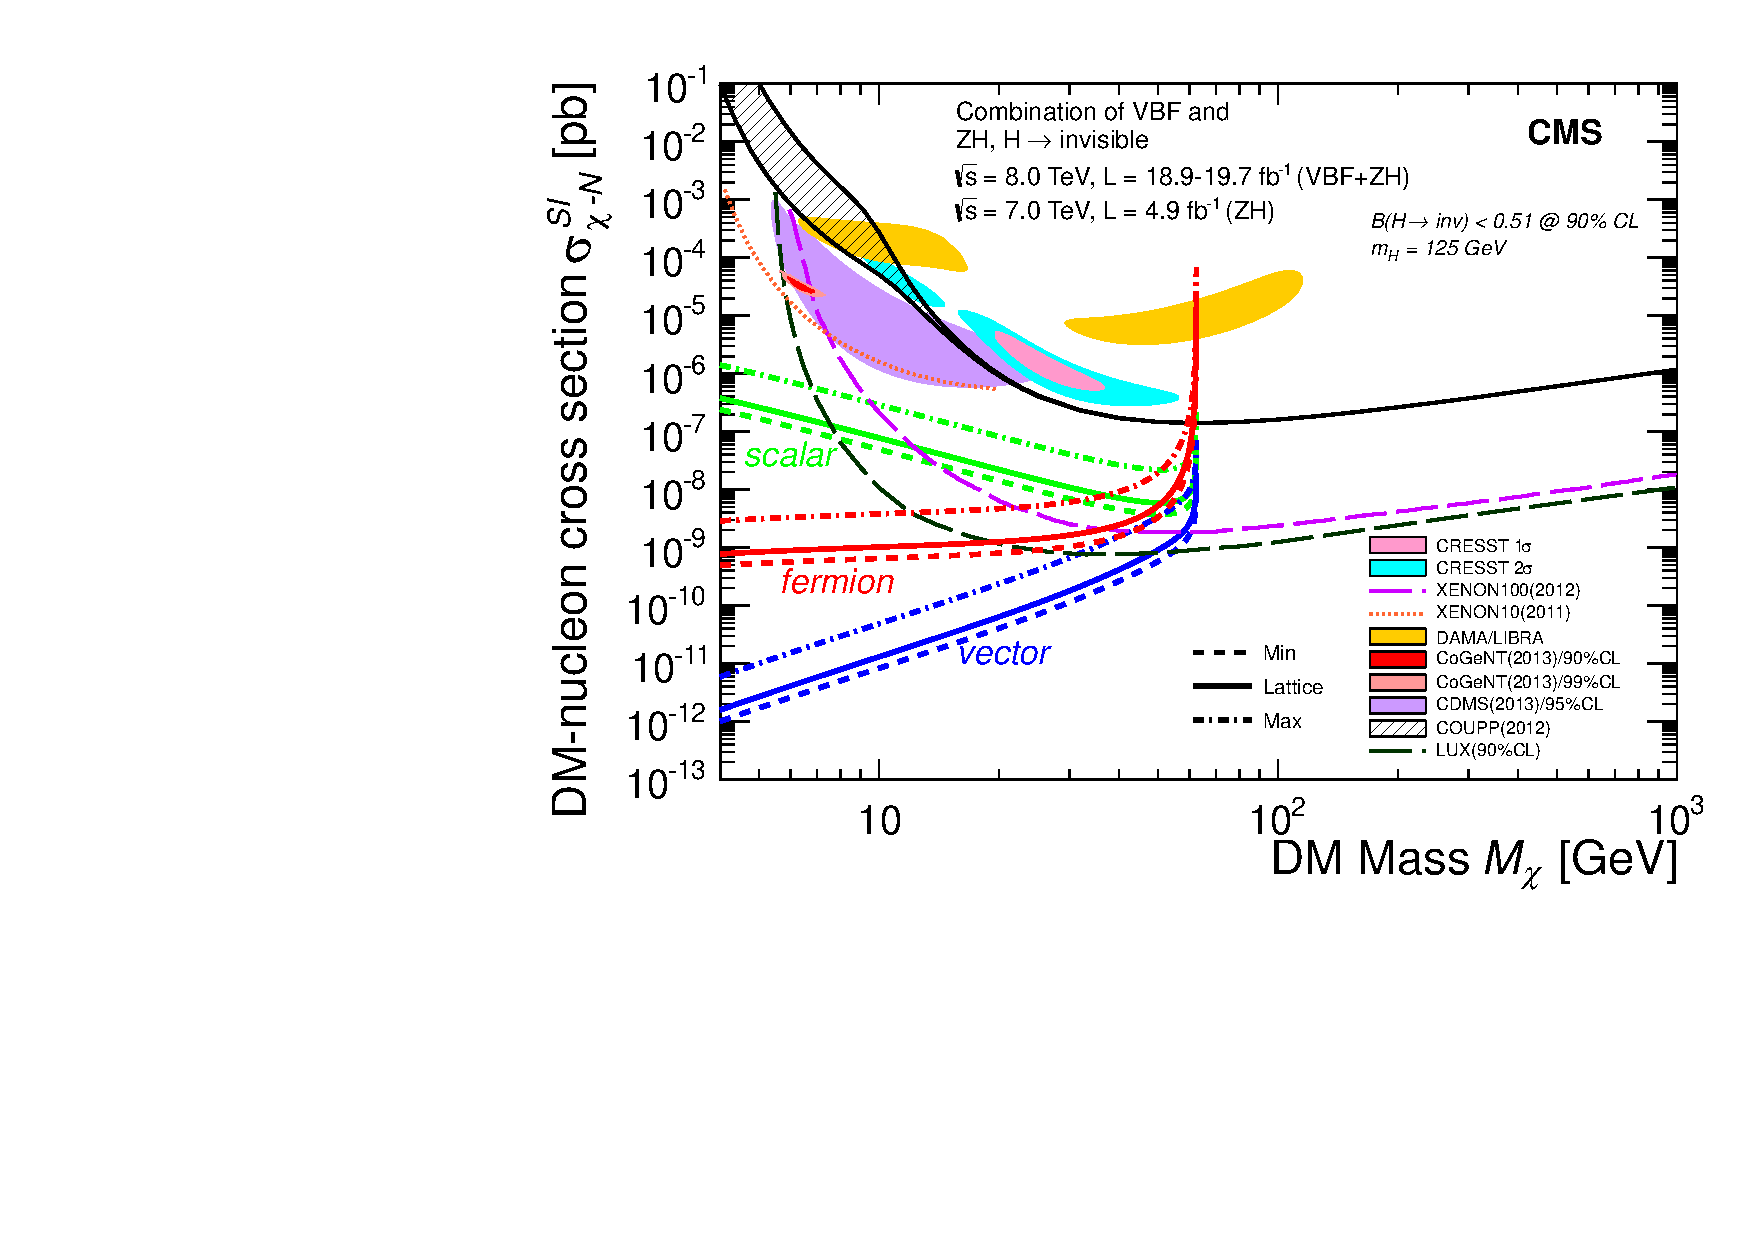
\includegraphics[clip=true,trim=0 0 0 0, width=.65\textwidth]{TalkPics/panicpics/dmlimit.pdf}    };
      \begin{scope}[x={(image.south east)},y={(image.north west)}]
        \draw[red,ultra thick,visible on=<2>] (0.,0.) -- (1,1);
        \draw[red,ultra thick,visible on=<2>] (0.,1.) -- (1,0);
      \end{scope}
    \end{tikzpicture}
  \end{frame}

  \begin{frame}%CHECK AT END
    \frametitle{Conclusions}
    \label{lastframe}
    \begin{columns}
      \column{.5\textwidth}
    \begin{block}{}
        \footnotesize
        \begin{itemize}
        \item %!!some conclusions
        \end{itemize}
      \end{block}
        \column{.5\textwidth}
          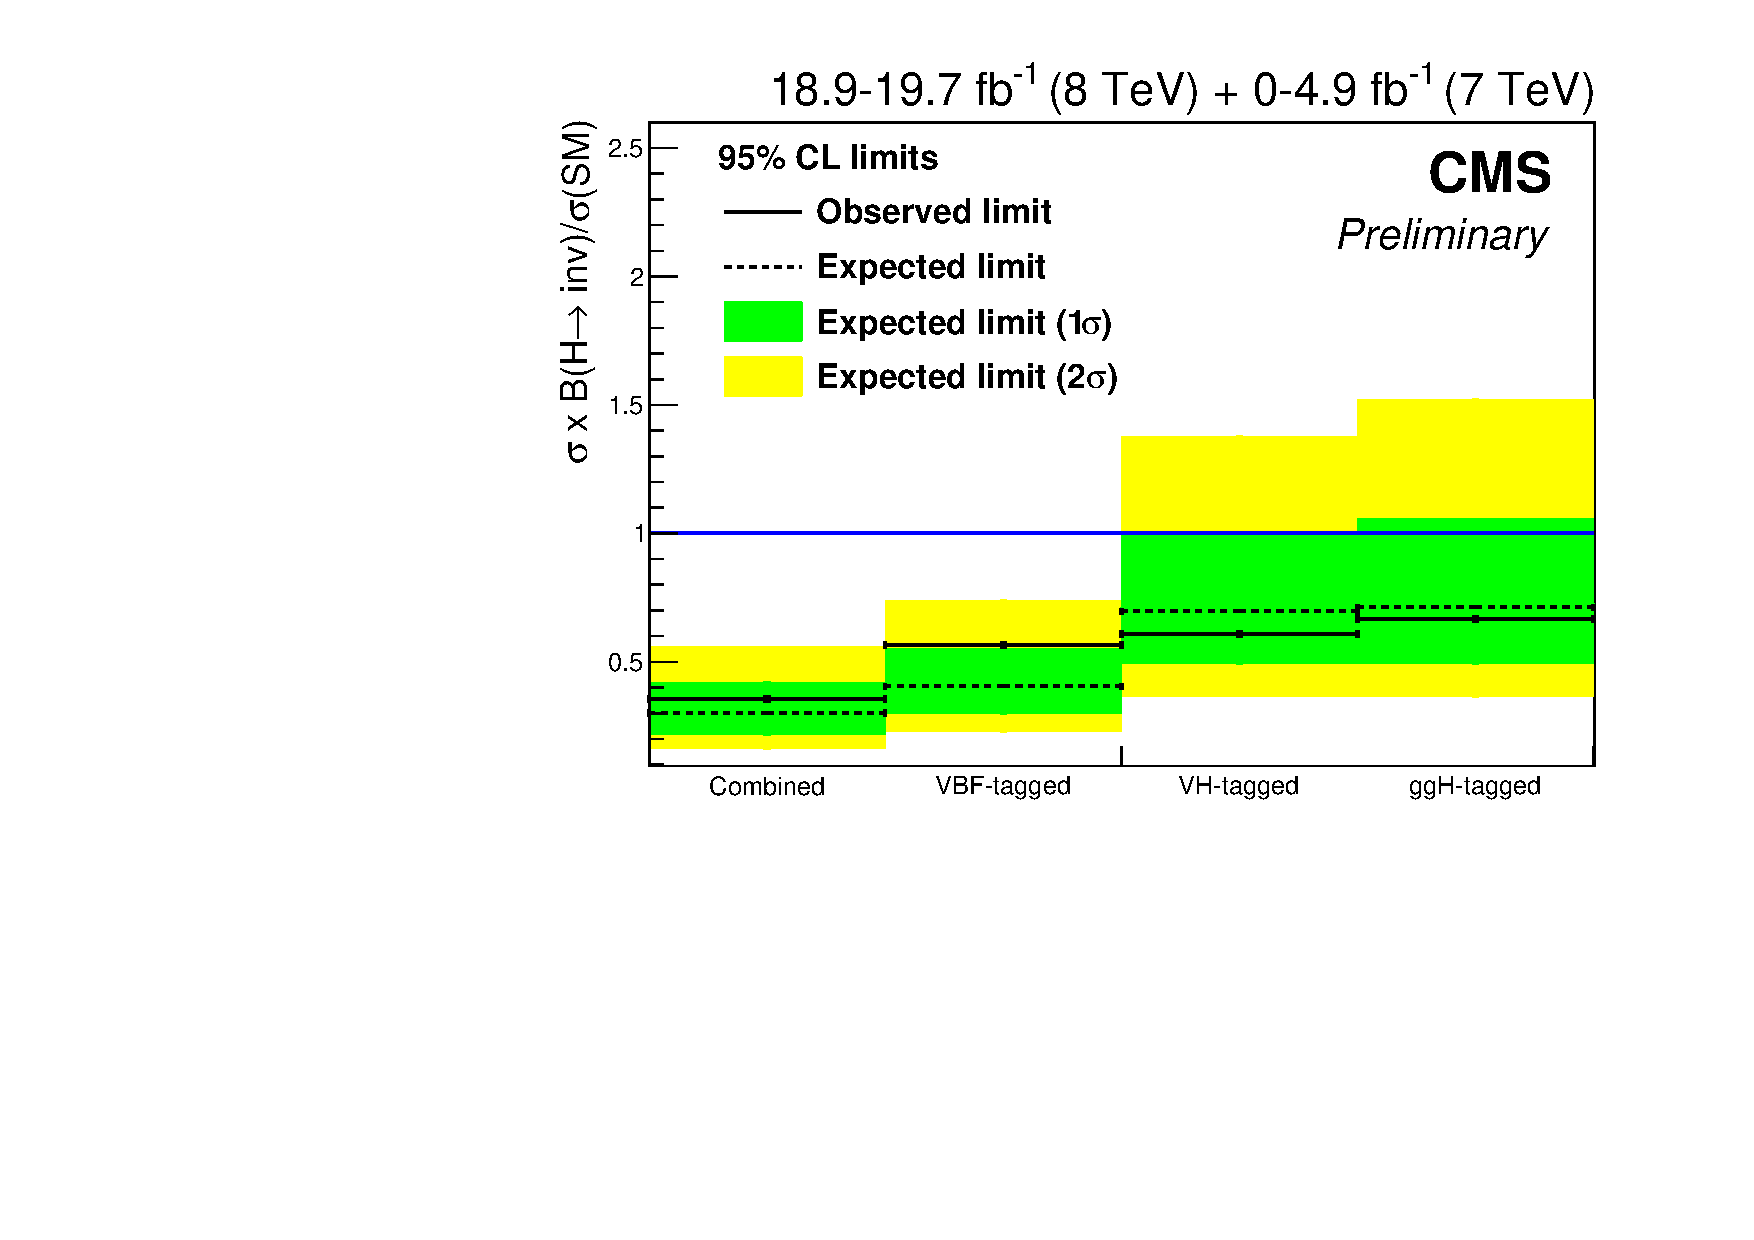
\includegraphics[clip=true,trim=0 0 0 0, width=1.2\textwidth]{TalkPics/studentseminar221015/hig15012figures/channellimit.pdf}

    \end{columns}


  \end{frame}

  \begin{frame}
    \frametitle{Backup}
  \end{frame}

\end{fmffile}
\end{document}

